\documentclass[12pt]{article}
\usepackage[utf8]{inputenc}
\usepackage{amsmath}
\usepackage{graphicx}
\usepackage[utf8]{inputenc}
\usepackage[T1]{fontenc}
\usepackage{natbib}
\usepackage{soul}
\usepackage{hyperref}
\usepackage{listings}
\usepackage{color}

\definecolor{codebg}{rgb}{0.95,0.95,0.95}
\definecolor{codeframe}{rgb}{0.8,0.8,0.8}

\lstset{
    backgroundcolor=\color{codebg},
    frame=single,
    frameround=tttt,
    rulecolor=\color{codeframe},
    basicstyle=\ttfamily,
    columns=fullflexible,
    breaklines=true
}

\title{Analiza statystyczna przyznawania funduszy UE gminom}
\author{Krzysztof Rudnicki, Michał Sar}
\date{\today}

\begin{document}

\maketitle

\tableofcontents

\begin{abstract}
    This is a brief summary of your study, its results, and major conclusions.
\end{abstract}


\section{Wstęp}
\paragraph{Kontekst}
W 2024 mija 20 lat od wstąpienia Polski do Unii Europejskiej \cite{1}. 
Od tamtej pory bilans Polski w stosunku do Brukseli wynosi 175 miliardów euro na 
plus dla Polski \cite{2} W samym 2023 roku Polska otrzymała z UE prawie 3.5 miliarda 
złotych, wpłacająć niecały miliard złotych \cite{3} W naszej pracy ponawiamy analizę 
statystyczną wykonaną sprzed 7 lat, na nowych danych, od początku roku 2014 do końca 
roku 2023
\paragraph{Cel}
Celem pracy jest sprawdzenie jakie dane na temat gminy najbardziej korelują z liczbą 
przyznanych funduszy Unii Europejskiej danej gminy
\paragraph{Hipoteza} 
\ul{Gęstość zaludnienia jest \textbf{najważniejszym} czynnikiem wpływającym na 
przyznanie środków unijnych} \\
\paragraph{Metoda badawcza}
\begin{enumerate}
    \item Zebrać dane UE
    \item Zebrać dane gmin
    \item Połączyć dane po numerze TERYT
    \item Przeanalizować dane 
    \item Wyświetlić wyniki
\end{enumerate}
\paragraph{Wyniki}

\section{Omówienie rozdziałów}
Na początku artykułu przedstawiamy czemu wybraliśmy taki temat, co chcemy osiągnąć 
naszą pracą, w jaki sposób chcemy to osiągnąć i jaki rezultat ostatecznie udało nam się 
pokazać \\  
Następnie opisujemy istniejącą literaturę na temat środków Unijnych z którą się 
zapoznaliśmy i przedstawiamy w czym różni się nasza praca od istniejących \\ 
Potem tłumaczymy nasz proces badawczy, w jaki sposób zbieraliśmy i łączyliśmy dane, 
jak je analizowaliśmy i jak przedstawialiśmy wyniki \\ 
Kontynując, pokazujemy co otrzymaliśmy ostatecznie w wyniku naszej pracy \\ 
Przedostatni rozdział zajmuje się dyskusją wyników, przedstawiamy co udało nam się 
osiągnać i dlaczego, czego nie udało nam się osiągnąć i dlaczego oraz przede wszystkim 
konfrontujemy wynik z naszą hipotezą \\ 
Na końcu podsumowujemy całą pracę i przedstawiamy spis literatury z której korzystaliśmy

\section{Opis literatury}
\paragraph{Decision trees: from efficient prediction to responsible AI}
Artykuł poświęcony jest omówieniu drzew decyzyjnych, rozpoczyna od zdefiniowania czym 
drzewo decyzyjne jest, jakie są jego unikalne cechy, gdzie jest stosowane, jakie ma wady 
i potencjalne zagrożenia oraz jak można je zminimalizować \cite{4} \\ 
Wybraliśmy ten artykuł gdyż opisuje jedną z głównych metod którą zamierzamy stosować w 
naszym procesise badawczym do przeanalizowania danych 
\paragraph{Application of Successful EU Funds Absorption Models to Sustainable Regional Development}
Artykuł wykorzystał ankiety pytając 244 osób o to jak 
efektywnie wykorzystywane były fundusze UE w Polsce, Słowenii, 
Węgrzech i Chorwacji. Artykuł podkreśla znaczenie możliwości 
technicznych, administracyjnych, koordynacji pomiędzy 
instytucjami i dobrymi mechanizmami nadzorowania funduszy 
europejskich jako kluczowe dla skutecznego wykorzystywania 
funduszy unijnych.  \cite{5} \\ 
Artykuł przydał się nam w ocenie jakie parametry pozytywnie wpływają na korzystanie z funduszy UE i jakie moglibyśmy śledzić w naszym modelu.
W naszym artykule zamiast ankiet wykorzystujemy dostępne już dane, a wyniki staramy się stworzyć przy użyciu modeli statystycznych. Dodatkowo zajmujemy się przedstawieniem jakie parametry wpływają na przyznanie środków UE a nie na to w jaki sposób można te środki skutecznie wykorzystywać 
\paragraph{It’s not about the money. EU funds, local opportunities, and Euroscepticism})
Artykuł opisuje jak pieniądze z Unii Europejskiej wpływają na eurosceptycyzm w danym kraju na podstawie Walii w kontekście referendum "Brexit". 
Badanie wykorzystuje metodę Regression discontinuity design (RDD), wybrano Walię z uwagi na różnicę w ilości pieniędzy przekazanych poszczególnym rejonom. 
Autorzy wykazali że sama ilość pieniędzy przekazana danemu 
regionowi nie zwiększa znacznie poparcia dla 
Unii Europejskiej, natomiast duże nakłady powiązane z 
widoczną, namacalną poprawą na lokalnym rynku wpływają 
pozytywnie na postrzeganie Unii Europejskiej w lokalnych 
społecznościach \cite{6} \\ 
Nasz artykuł koncentruje się na tym co wpływa na przyznanie funduszy unijnych a nie na samą reakcje na ich przyznanie 
\section{Proces badawczy}
Proces badawczy podzieliliśmy na 3 zasadnicze etapy, zebranie danych, przeanalizowanie ich i zaprezentowanie wyników

\paragraph{Zbieranie danych}
Wszystkie dane pobieraliśmy ze strony GUS-u \\
\href{https://bdl.stat.gov.pl/bdl/start}{https://bdl.stat.gov.pl/bdl/start} \\ 
Dane wybieraliśmy z zakładki "Popularne podgrupy", następnie wybieraliśmy wszystkie lata które nas 
interesowały (od 2014 do 2023 roku włącznie), po przejściu dalej wybieraliśmy wszystkie gminy, 
finalnie otrzymując tablicę którą pobieraliśmy do formatu csv \\ 
\begin{figure}[h]
    \caption{Strona z gusy z zaznaczonymi podgrupami z których korzystaliśmy}
    \centering
    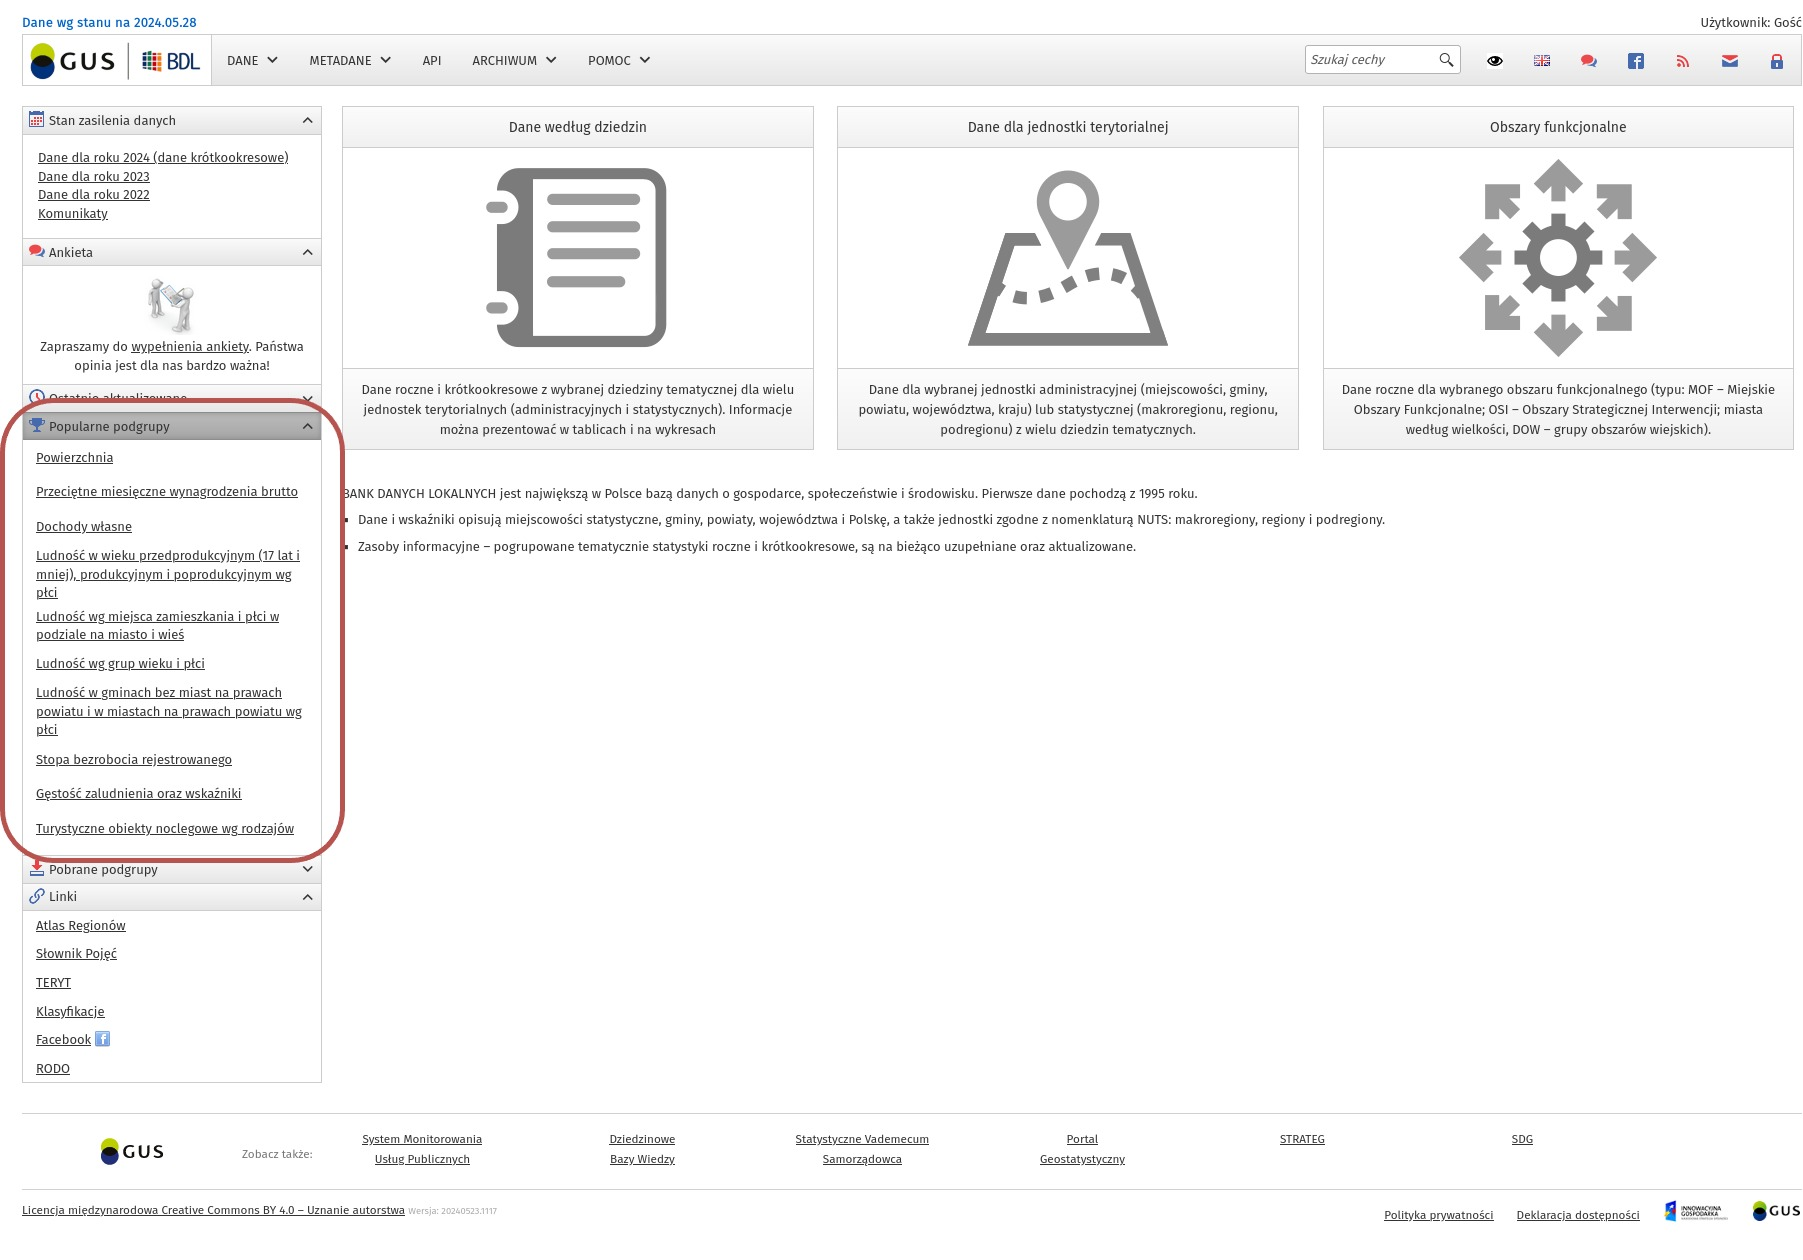
\includegraphics[width=1.0\textwidth]{gus}
    \end{figure}
\begin{figure}[h]
    \caption{Strona z gusy z zaznaczonymi podgrupami z których korzystaliśmy}
    \centering
    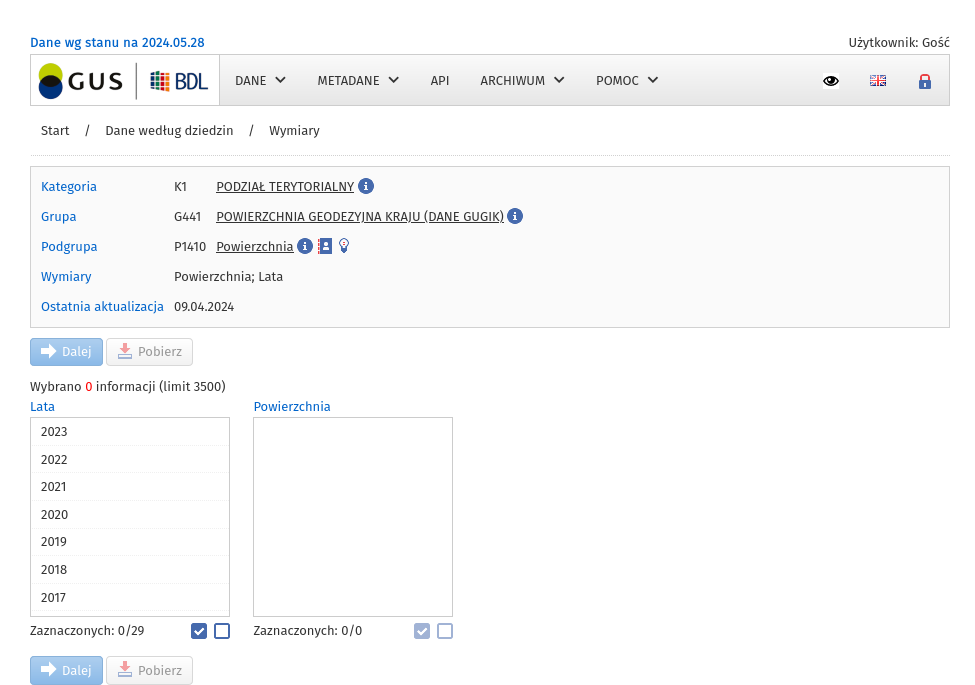
\includegraphics[width=1.0\textwidth]{dane2}
\end{figure}
\begin{figure}[h]
    \caption{Strona z gusy z zaznaczonymi podgrupami z których korzystaliśmy}
    \centering
    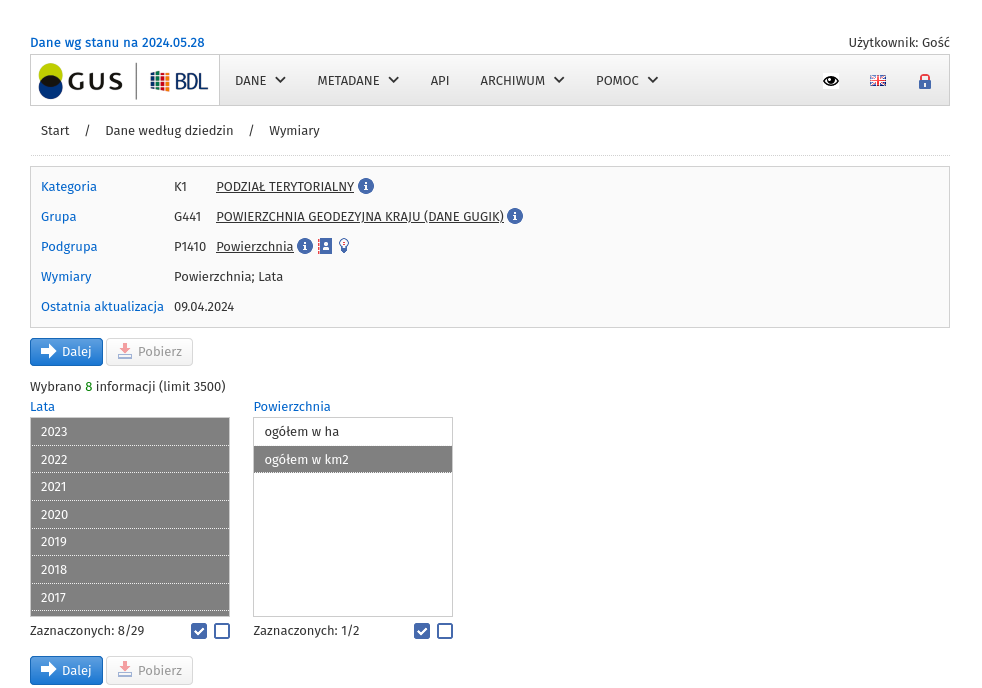
\includegraphics[width=1.0\textwidth]{dane3}
\end{figure}
\begin{figure}[h]
    \caption{Strona z gusy z zaznaczonymi podgrupami z których korzystaliśmy}
    \centering
    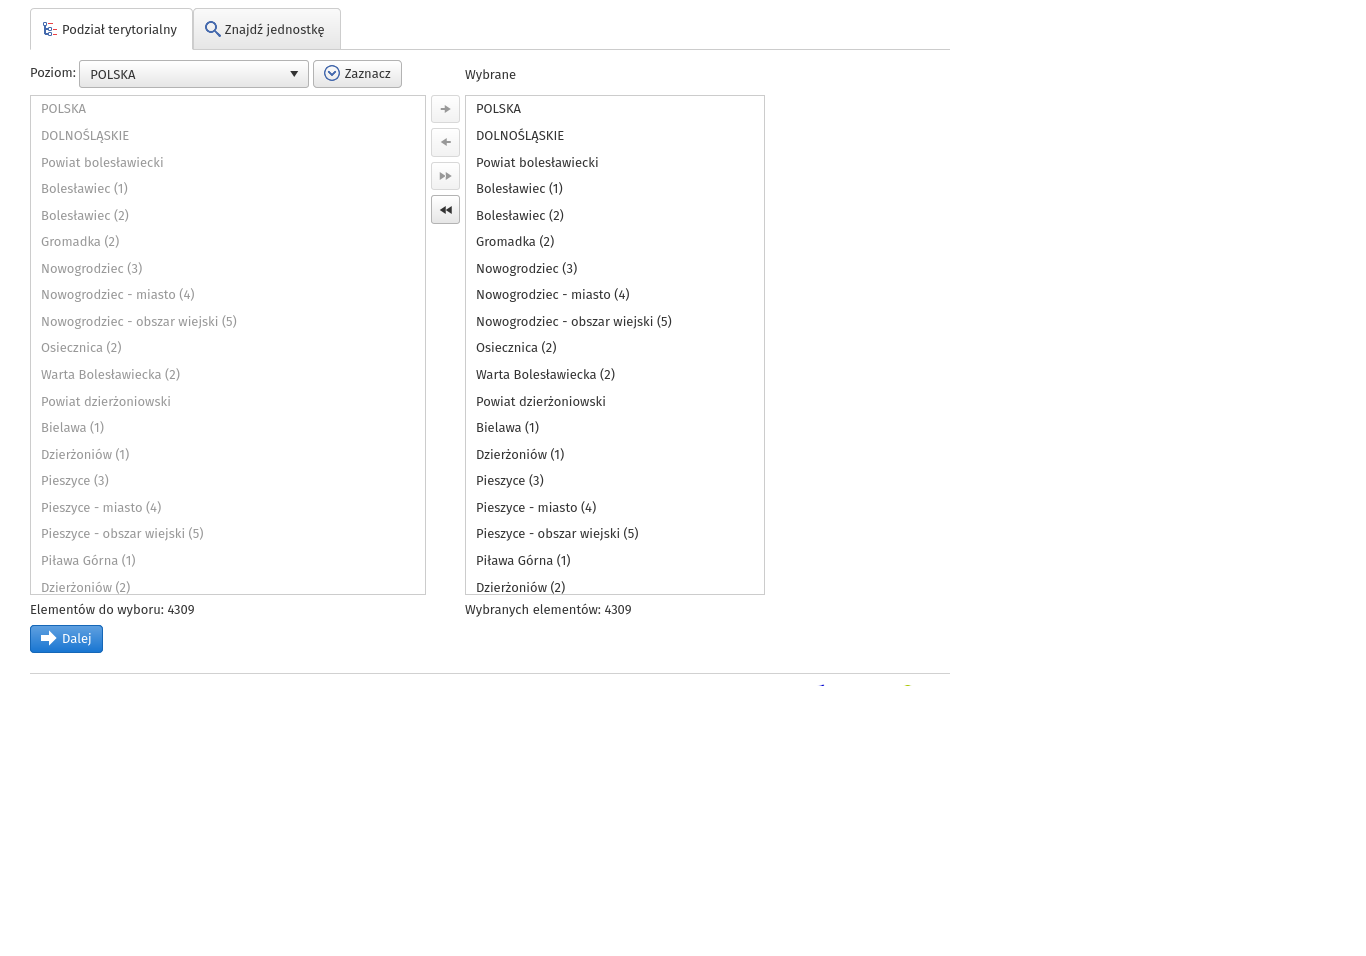
\includegraphics[width=1.0\textwidth]{dane4}
\end{figure}
\begin{figure}[h]
    \caption{Strona z gusy z zaznaczonymi podgrupami z których korzystaliśmy}
    \centering
    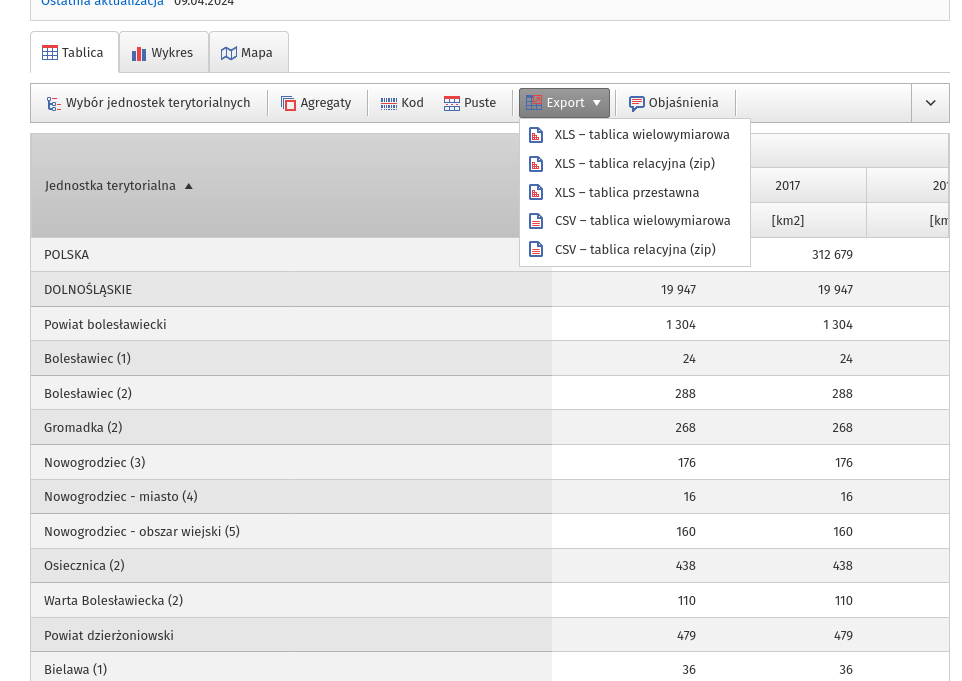
\includegraphics[width=1.0\textwidth]{dane5}
\end{figure}

\paragraph{Przygotowywanie danych}
Dane musieliśmy przeprocesować przed ich wykorzystaniem, przede wszystkim usuwaliśmy wszelkie wiersze zawierające wartości puste lub NULL
\section*{Description of Code}

The provided Python code snippet is part of a Jupyter Notebook. Its main functionality is to calculate and display the feature importance of a trained machine learning model. Feature importance is a key metric in understanding which features (or input variables) have the most significant impact on the model's predictions. Here's a breakdown of what the code does:

\begin{enumerate}
    \item It creates a dictionary, \texttt{feature\_importance}, which maps feature names to their respective importance scores as determined by the model.
    \item The dictionary is then sorted by importance scores in descending order.
    \item Finally, the code iterates through the sorted dictionary and prints out each feature's importance score alongside the feature's name.
\end{enumerate}

The code snippet provided is as follows:

\begin{lstlisting}[language=Python]
feature_importance = dict(zip(feature_names, model.feature_importances_))
for feature, importance in sorted(feature_importance.items(), key=lambda x: x[1], reverse=True):
    print(f'{importance:.5f} — {feature}')
\end{lstlisting}

\section*{Data Processed}

The code processes the following types of data:
\begin{itemize}
    \item \texttt{feature\_names}: A list of feature names used in the model.
    \item \texttt{model.feature\_importances\_}: An array of feature importance scores generated by the model.
\end{itemize}

The purpose of this data processing is to identify and rank the most influential features in the model, which can be useful for feature selection, model interpretation, and improving model performance.

\end{document}
\paragraph{Analiza danych}

\paragraph{Przedstawienie wyników}

\section{Wyniki}


\section{Dyskusja}


\section{Konkluzja}


\bibliographystyle{plain}
\bibliography{references}

\end{document}
